\documentclass{article}

% Language setting
% Replace `english' with e.g. `spanish' to change the document language
\usepackage[spanish]{babel}
\usepackage[numbers]{natbib}


% Set page size and margins
% Replace `letterpaper' with `a4paper' for UK/EU standard size
\usepackage[a4paper,top=2cm,bottom=2cm,left=3cm,right=3cm,marginparwidth=1.75cm]{geometry}
\setlength{\parindent}{0pt}


% Useful packages
\usepackage{amsmath}
\usepackage{graphicx}
\usepackage[colorlinks=true, allcolors=blue]{hyperref}
\usepackage{xcolor}
\usepackage{listings}
\usepackage{float}



\title{Manual de Usuario de ATLAS}
\author{Maria del Valle Alonso de Caso Ortiz}

\begin{document}
\maketitle

%\begin{abstract}
%Your abstract.
%\end{abstract}

%%--------------------------------------------------------

\section{Introducción a ATLAS.}

ATLAS es una aplicación de software gratuita, de código abierto y basada en web, desarrollada por la comunidad OHDSI para apoyar el diseño y la ejecución de análisis observacionales con el fin de generar evidencia del mundo real a partir de datos observacionales a nivel de paciente. \\

ATLAS es una plataforma de análisis de ciencia abierta que se puede instalar localmente dentro de su institución para realizar análisis en una o varias bases de datos observacionales que se han estandarizado al Modelo de Datos Común OMOP V5 y puede facilitar el intercambio de diseños de análisis con cualquier otra organización dentro de la comunidad OHDSI que haya adoptado los mismos estándares y herramientas de ciencia abierta \cite{OHDSIAtlasWiki}


%%-------------------------------------------------------

\section{Despligue de la herramienta.}

ATLAS puede desplegarse de múltiples maneras, desde formas muy sencillas que no necesitan ninguna instalación local hasta la implementación local más pura y compleja. En este manual de usuario se presentan todas las formas de implementar ATLAS de menor a mayor complejidad.

\subsection{ATLAS demo}

ATLAS demo es una instanciación, disponible públicamente online de forma gratuita, que permite acceder a una versión demo de la herramienta. Es la forma más fácil de tener un primer contacto con la herramienta, pues solo es necesario acceder a través del  \href{https://atlas-demo.ohdsi.org/}{link} que nos facilita la página web oficial de OHDSI, desde la pestaña \href{https://atlas-demo.ohdsi.org/}{software tools}. \\

\begin{figure}[H]
    \centering
    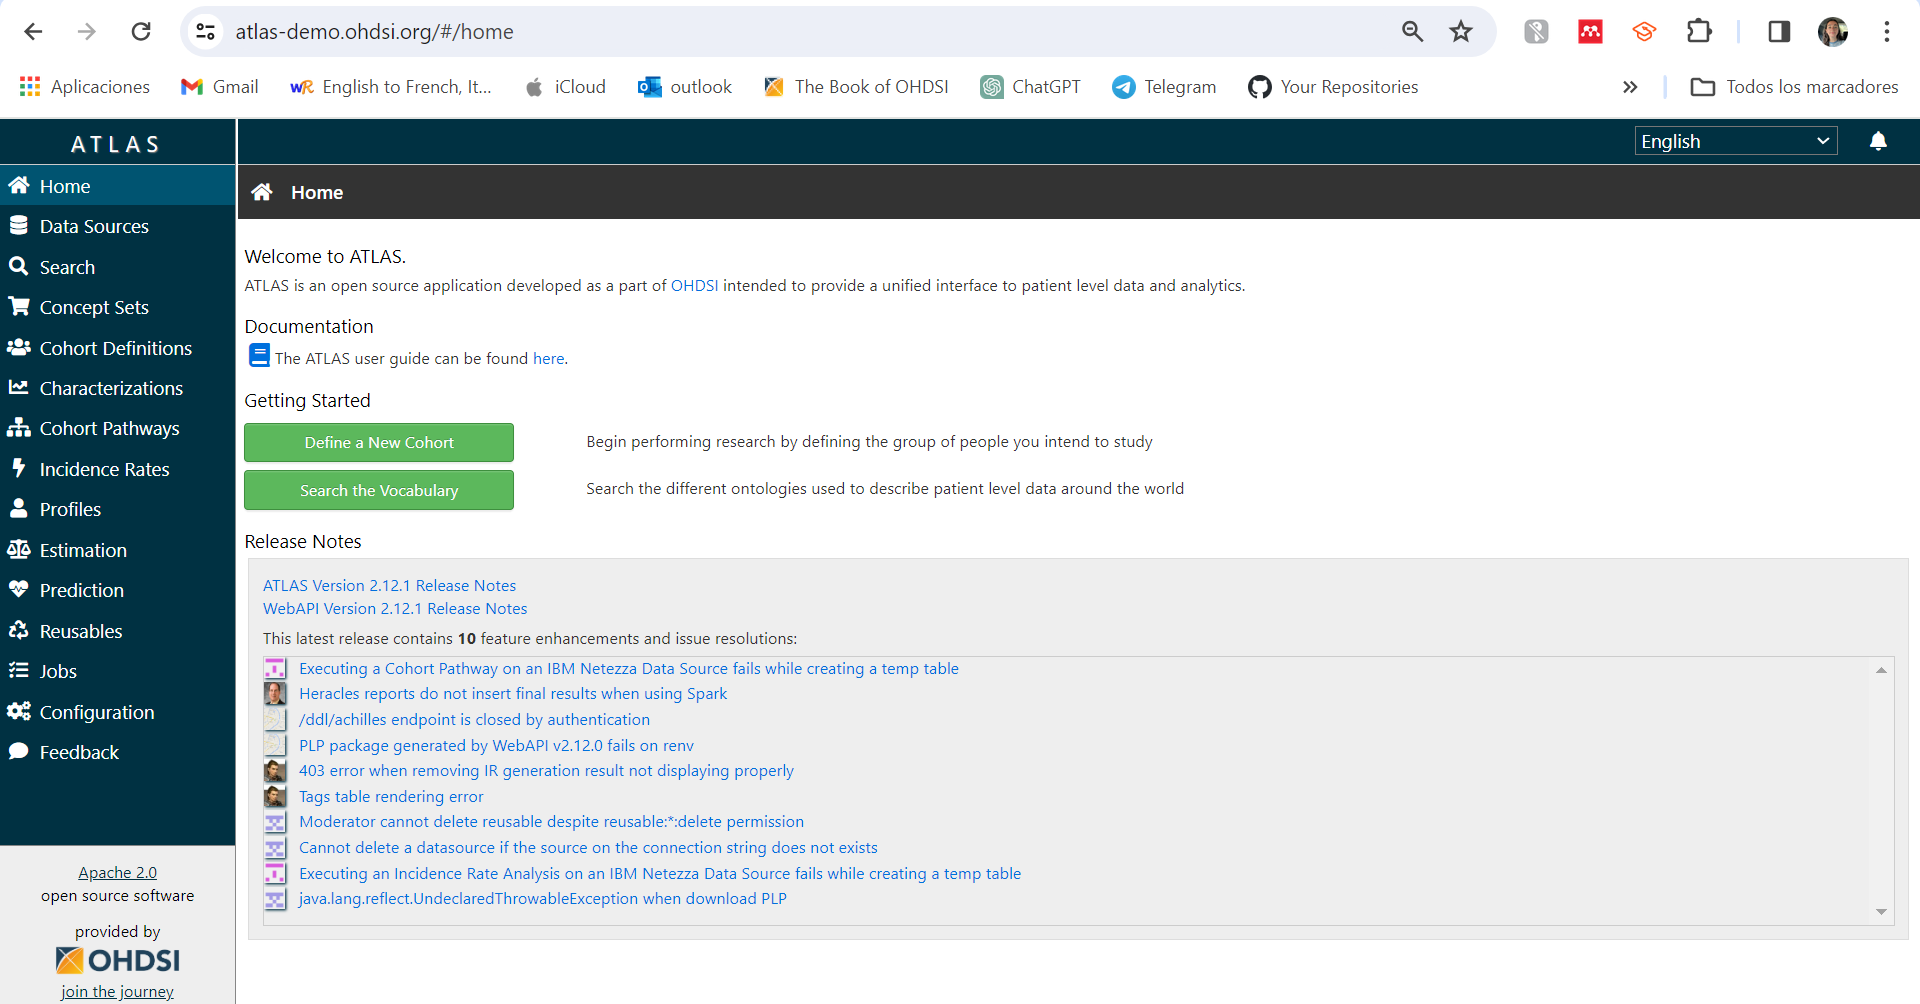
\includegraphics[width=0.90\textwidth]{images/atlasDemo.png}
    \caption{Captura de pantalla de menú principal de ATLAS demo}
\end{figure}

A pesar de ser una demo, no debemos subestimar su potencial de operación. Esta versión online de la herramienta, ofrece soporte para cuatro bases de datos (demo) de OHDSI: ATLASPROD, Common Evidence Model, SYNPUF 1K y SYNPUF 5\%. Además, al ser una herramienta disponible online públicamente para cualquier usuario, almacena la información que deposita cada usuario tras su uso, es decir, almacena gran cantidad de ejemplos de estructuras de cohortes, caracterización... aunque hay que tener en cuenta que al ser estructuras definidas por usuarios no administradores, pueden ser incorrectas. No obstante, no deja de ser un gran repositorio público para empezar a trabajar con ATLAS. \\

\begin{figure}[H]
    \centering
    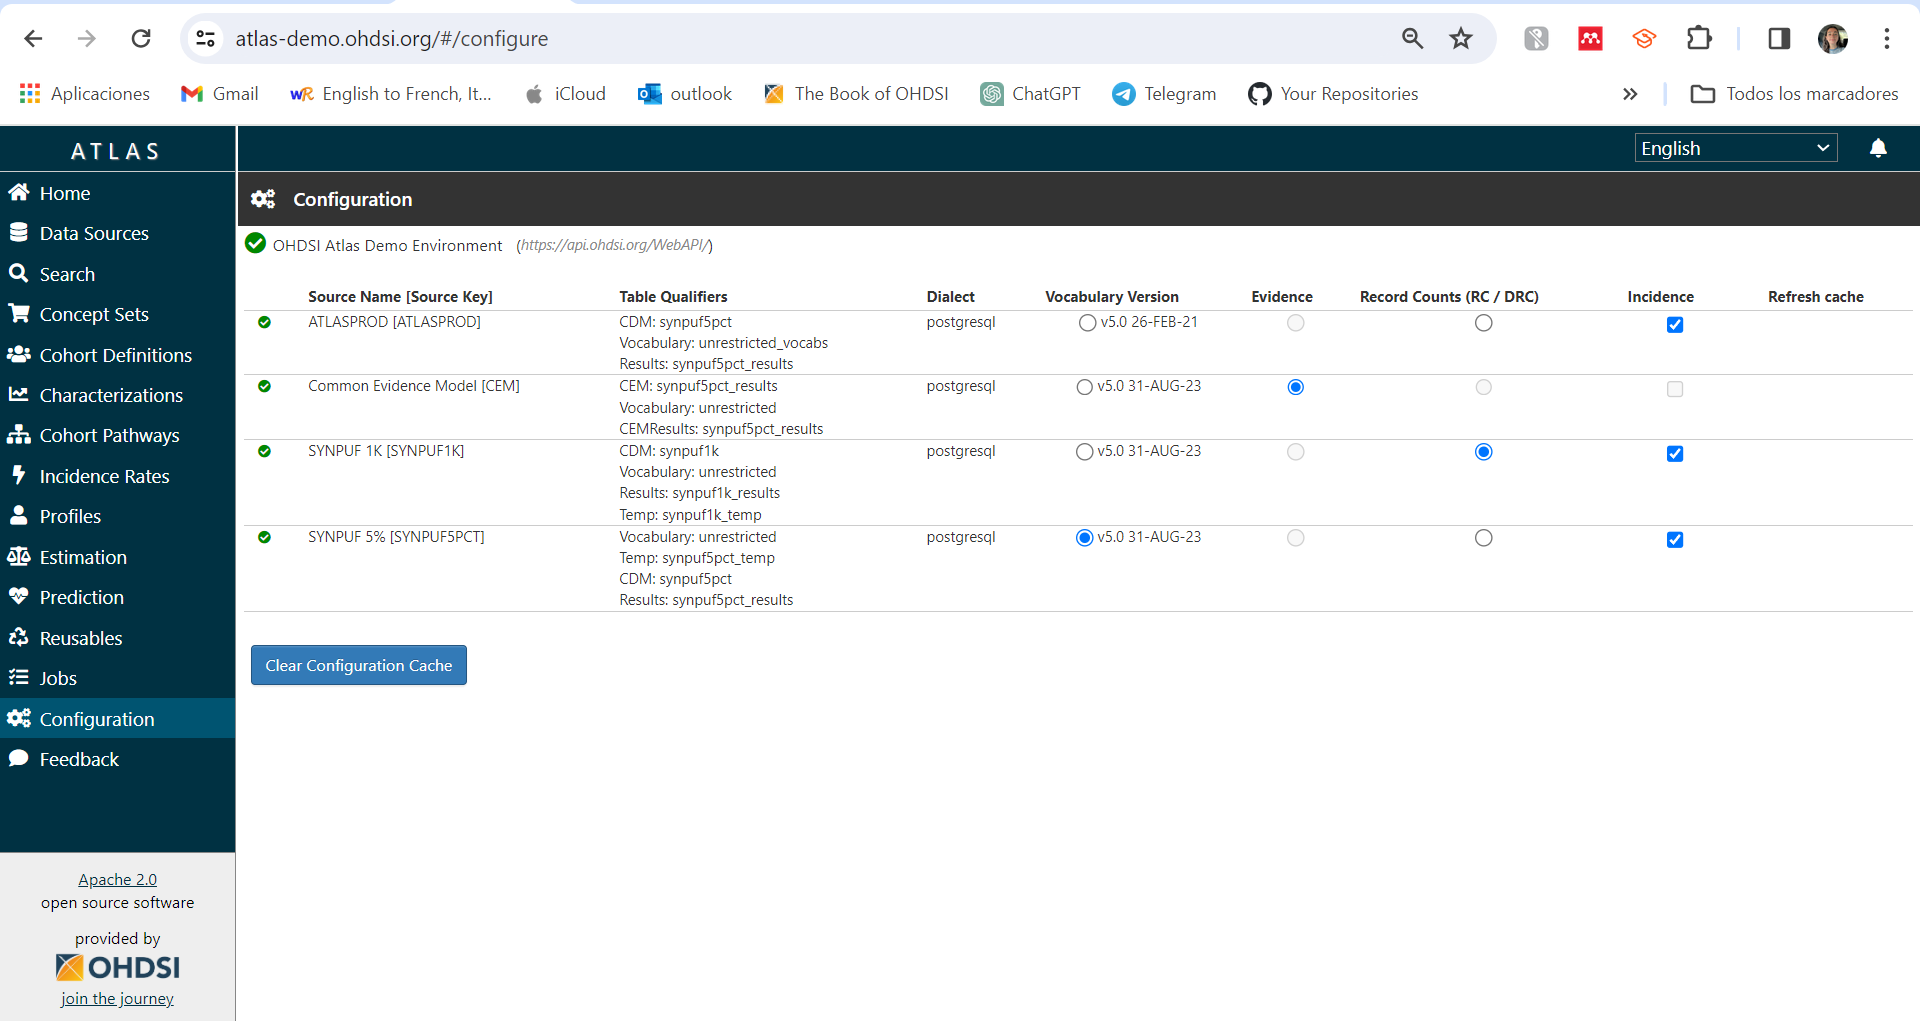
\includegraphics[width=0.90\textwidth]{images/atlasDemo(1).png}
    \caption{Captura de pantalla de bases de datos que utiliza ATLAS demo}
\end{figure}

\begin{figure}[H]
    \centering
    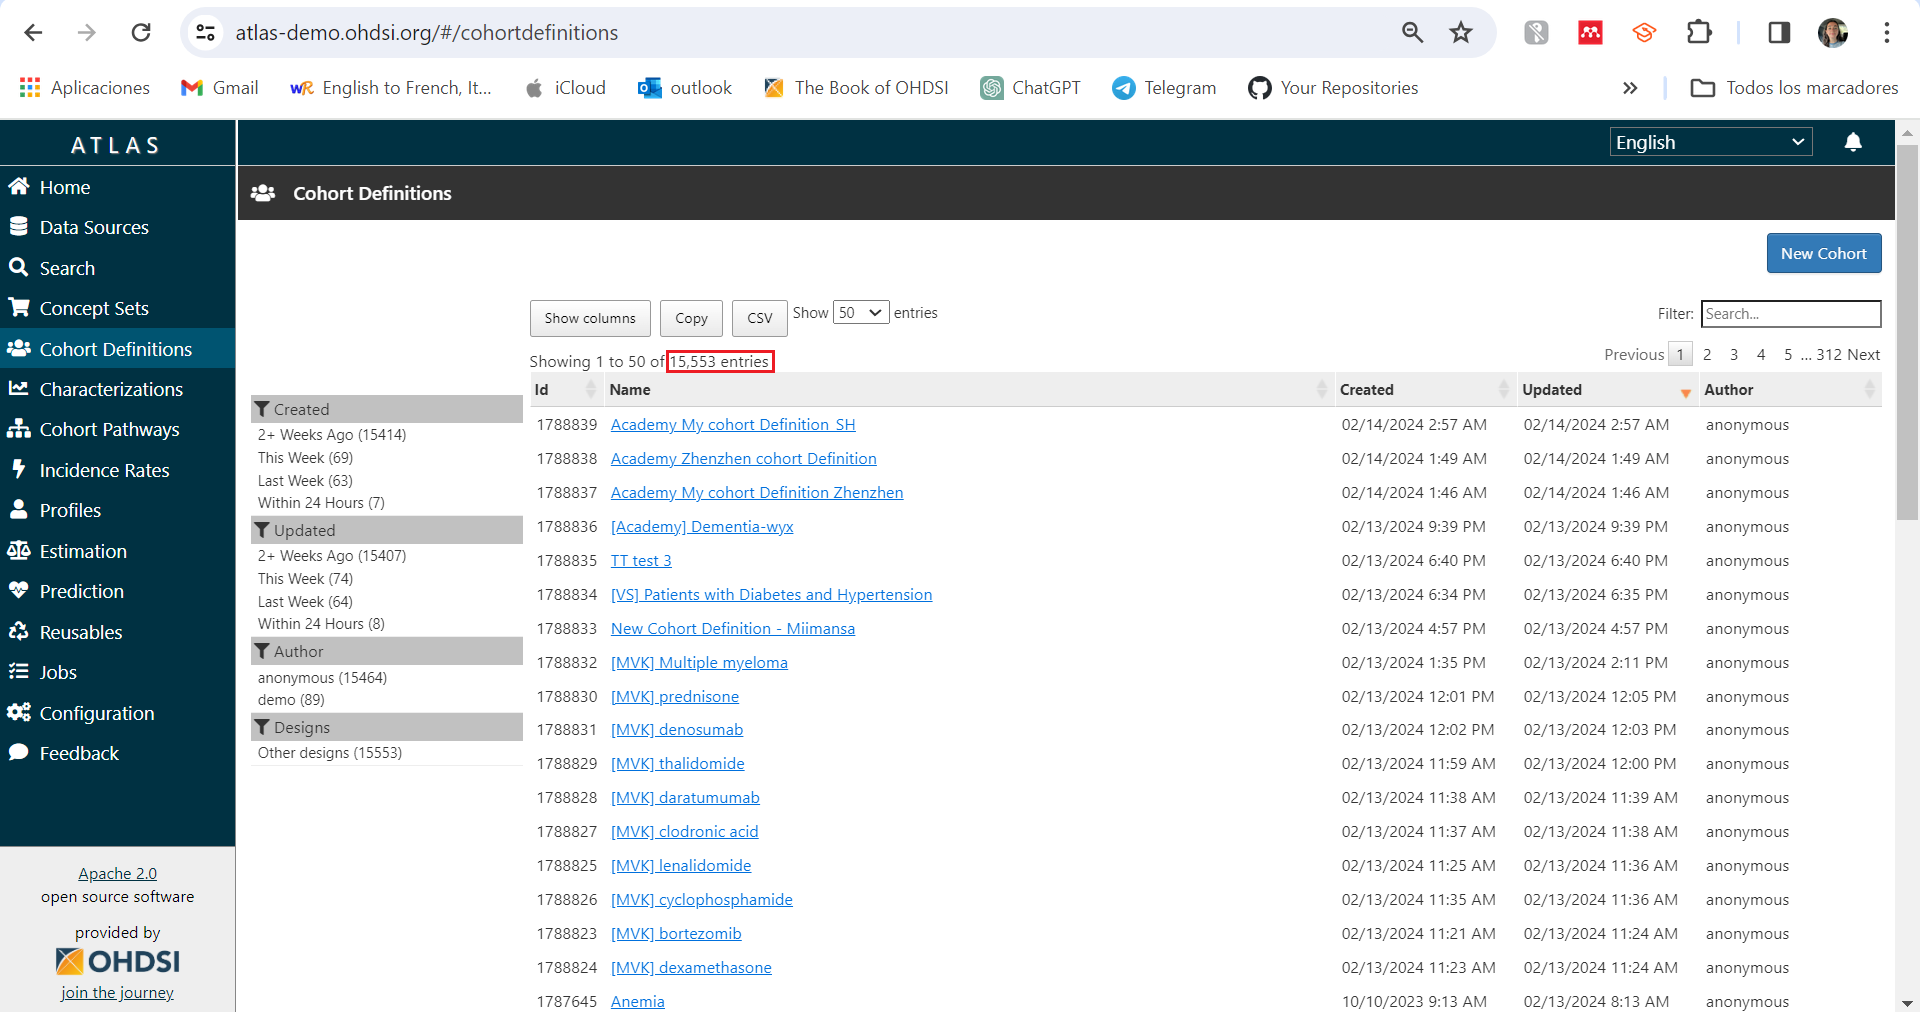
\includegraphics[width=0.90\textwidth]{images/atlasDemo(2).png}
    \caption{Captura de pantalla señalando el número de entradas de definición de cohorte que almacena ATLAS demo}
\end{figure}


Frente a este despliegue online, sin necesidad de descargar ni instalar ningún programa ni software adicional, se encuentra la opción de desplegar la herramienta de manera local, para limpiar la herramienta de todos estos datos de otros usuarios y trabajar localmente con información propia. \\

Sin embargo, esta instalación puede llegar a ser bastante compleja puesto que hay muchos componentes con dependencias que deben ser considerados y configuraciones que deben ser establecidas. Por esta razón, dos iniciativas han desarrollado estrategias integradas de implementación que permiten instalar toda la pila como un paquete, utilizando algunas formas de virtualización: Broadsea \ref{cap:AtlasBroadsea} y Amazon Web Services (AWS) \ref{cap:AtlasAWS}. \cite{TheBookOfOhdsi}

\newpage
\subsection{ATLAS docker - Broadsea}\label{cap:AtlasBroadsea}

Broadsea es un proyecto basado en Docker que permite desplegar de manera consistente aplicaciones web de OHDSI (Atlas, Ares y Hades) junto con las dependencias de base de datos y redes necesarias para ejecutar esas herramientas. Broadsea ha permitido a los investigadores experimentar con herramientas de OHDSI sin necesidad de tener una experiencia técnica significativa o incurrir en gastos elevados. Debido al enfoque basado en Docker, la configuración es consistente, independientemente del sistema operativo o hardware.  \cite{Broadsea3.0}

\subsubsection{Despliegue}

El despliegue de ATLAS en Docker es muy sencillo y está bien documentado en el  \href{https://github.com/OHDSI/Broadsea}{repositorio de github} de Broadsea. De hecho, la propia organización considera Broadsea la manera más sencilla de instalar (y actualizar) Docker. Igualmente, en este manual detallaremos nuevamente los pasos para la configuración y despliegue de la herramienta.\\

\textbf{Requisitos para el despliegue}
\begin{enumerate}
    \item Descargar e instalar Docker. Lo más sencillo es seguir las instrucciones de la \href{https://docs.docker.com/engine/install/}{página web oficial} para la descarga y seguir la configuración por defecto para la instalación.
    
    \item Descargar e instalar Git. Lo más sencillo es seguir las instrucciones de la \href{https://git-scm.com/downloads}{página web oficial} para la descarga y seguir la configuración por defecto para la instalación.
\end{enumerate}

\textbf{Deployment}
\begin{enumerate}
    \item El primer paso para desplegar ATLAS es clonar localmente el repositorio de GitHub de Broadsea. Una forma rápida de hacerlo es, desde la terminal, introducir la siguiente línea.

\begin{lstlisting}[language=sh]
        git clone https://github.com/OHDSI/Broadsea.git
\end{lstlisting}

    \item El segundo paso, es desplegar el contenedor docker. Para ello, desde la terminal, nos situamos en la carpeta donde se ha copiado el repositorio de github de Broadsea. Podemos utilizar el comando cd con la ruta al repositorio local.

\begin{lstlisting}[language=sh]
        cd ruta\del\repositorio\Broadsea\local
\end{lstlisting}

    Una vez nos encontramos en la carpeta raíz del repositorio, ejecutamos el siguiente comando, que instalará el contenedor docker en nuestro ordenador.

\begin{lstlisting}[language=sh]
    docker compose pull && docker-compose --profile default up -d
\end{lstlisting}

    \item Para acceder a Broadsea basta con introducir la dirección IP: 127.0.0.1 en nuestro buscador web (Chrome recomendado).

\begin{figure}[H]
    \centering
    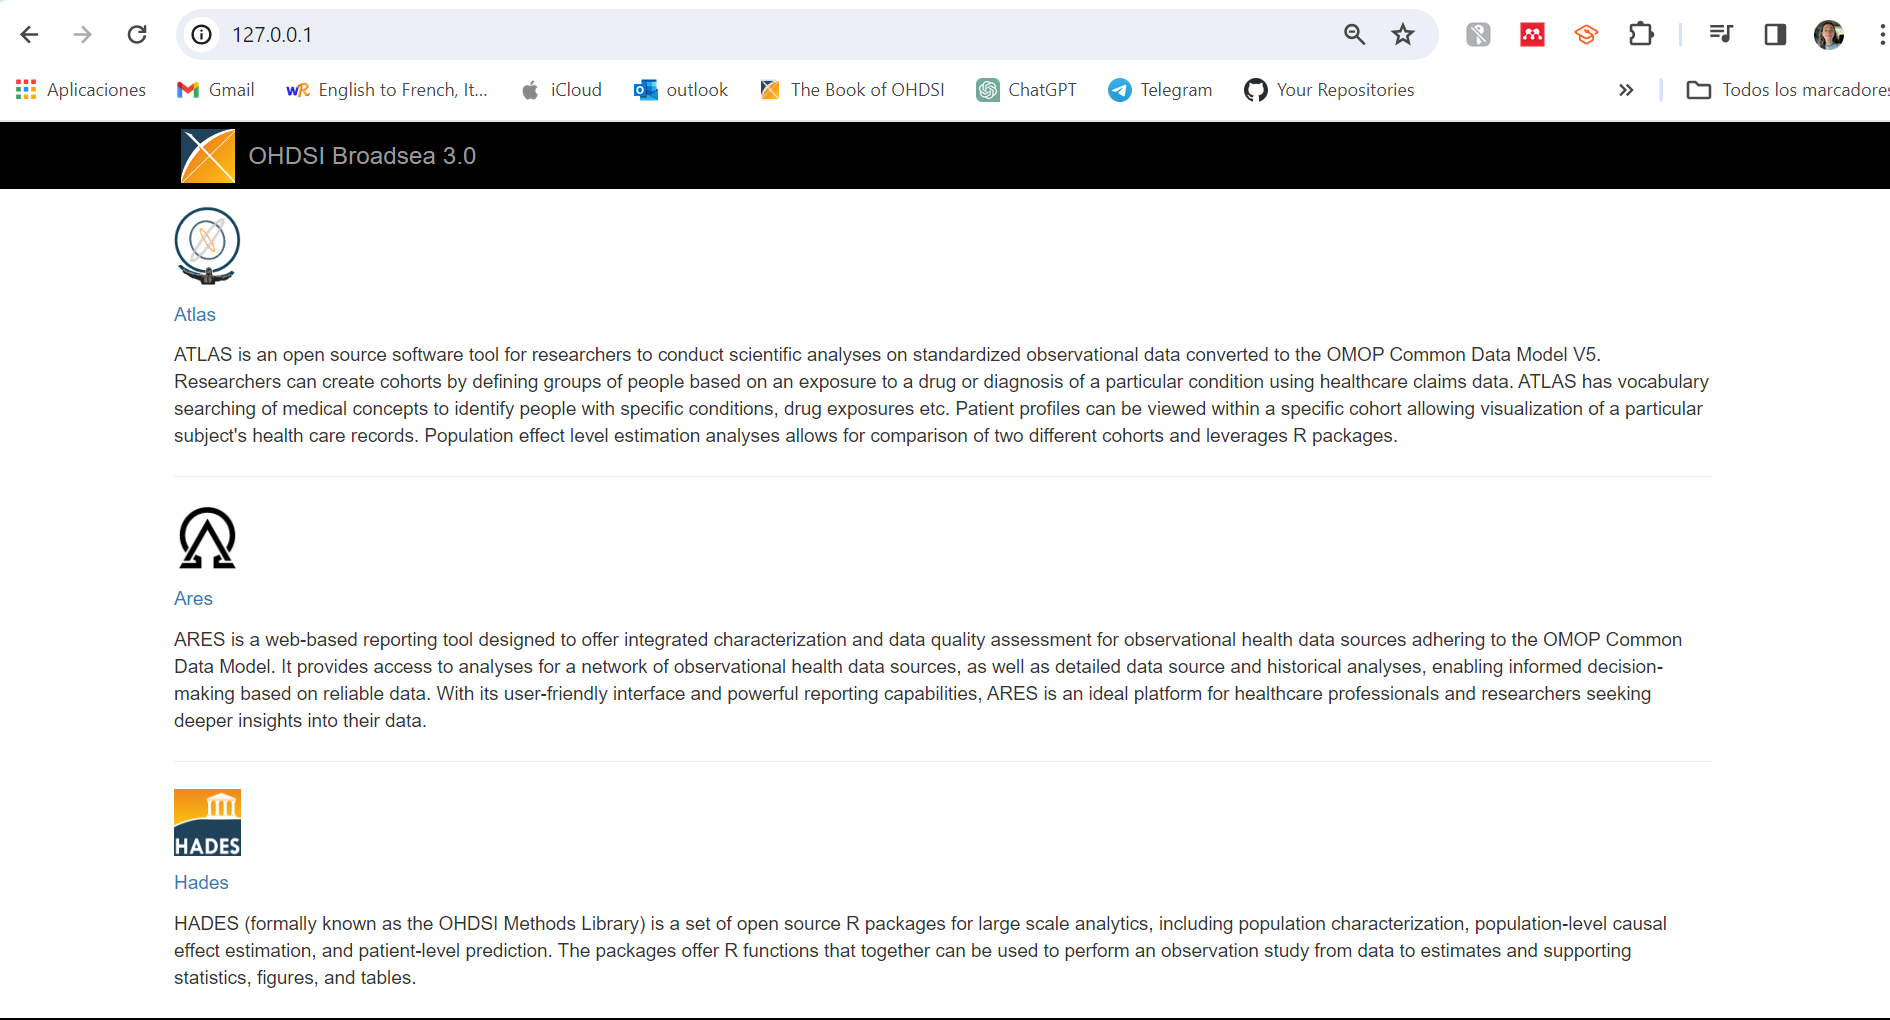
\includegraphics[width=0.90\textwidth]{images/broadseaCap.png}
\end{figure}


    



\end{enumerate}




\textcolor{red}{-----> Conectarse a la BD de BROADSEA <-----}










%%---------------------------------------------------
\newpage
\subsection{ATLAS AWS}\label{cap:AtlasAWS}

\textcolor{red}{https://github.com/OHDSI/OHDSIonAWS?tab=readme-ov-file}

\textcolor{red}{- OHDSI-in-a-box versión AWS}

\textcolor{red}{- OHDSIonAWS}


\subsection{ATLAS local }

La instalación local de ATLAS es la más compleja de todas porque requiere instalar todo el entorno de variable y configuraciones del sistema en el ordenador personal de forma manual. No obstante todo este proceso está correctamente documentado en las wikis de github \cite{AtlasSetup} y en el curso de EHDEN Academy \cite{EHDENAcademy} ''Infraestructure''. Para realizar la instalación de ATLAS localmente debemos seguir los siguientes pasos:

\begin{enumerate}
    \item Instalación de la WebAPI
    \item Instalación de ACHILLES
    \item Instalación de NodeJS
\end{enumerate}


%------------------------------------------------------
\newpage
\section{Funcionamiento de la herramienta.}




%%%%%%%%%%%%%%%%%%%%%%%%%%%%%%%%%%%%%%%%%%%%%5
\newpage
\bibliographystyle{plainnat}
\bibliography{sample}

\end{document}